\documentclass{llncs}
\usepackage[utf8]{inputenc}
\usepackage[english]{babel}
\usepackage{hyperref}

\pagestyle{plain}

\newcommand{\liquidsoap}{Liquidsoap}
\newcommand{\savonet}{Savonet}
\newcommand{\eg}{e.g.~}
\newcommand{\cf}{cf.~}
\newcommand{\TODO}[1]{\marginpar{#1}}

\usepackage{graphicx}

\title{Design of a Modular Programming Language for Generating Multimedia Streams: Liquidsoap}
\author{David Baelde \and Romain Beauxis \and Samuel Mimram}

\hypersetup{
  pdftitle={\csname @title\endcsname},
  pdfauthor={David Baelde, Romain Beauxis and Samuel Mimram},
  unicode=true,
  colorlinks=true,
  linkcolor=black,
  citecolor=black,
  urlcolor=black
}

\begin{document}
\maketitle

% \section*{Introduction}
The widespread of broadband Internet access and digital media during the last
decade has attracted a lot of attention on their potential applications.
Classical devices from the analog era, such as television, radio broadcasting
and phone communications are being adapted to the digital world. Additionally,
whilst analog applications were mostly based on hardware implementations, their
digital counterpart often consist in software implementations, \eg{} hardware
PBX for phone communications being replaced by software like Asterisk and IP
phones. These software implementations usually offer much more flexibility and
modularity in their design.
% and allow updates, both for bugfix and new features, at virtually no cost.

In this context of improvements, updates and enhancements of old technologies,
we are here specificaly interested in adapting audio and video broadcasting
techniques to the digital world. Creating and broadcasting a stream of
multimedia data with recent computers has become technically very easy. However,
the software technologies available to perform such tasks have not yet brought
the new ideas which are necessary in order to benefit from the new possibilities
offered by modern computing devices.

Designing a generator form multimedia streams needs a lot of flexibility in
order to be able to cope with most of the expectations and requirements of
users. For instance, a radio stream may have jingles announcing next coming
shows or commercials. It may also play those jingles at a regular interval of
time, between songs or on top of them. Also, a radio program may be composed of
automatic playlist for a certain period, \eg{} during the night, and live shows
during the day. Similarly, one may want to control and process the data before
broadcasting it to the public, performing tasks like
\begin{itemize}
 \item volume normalization,
 \item cross-fading between tracks, possibly parameterized by the respective
   volumes of the old and new tracks or predefined settings,
 \item remove blanks, either in automatic file streams or during live shows,
 \item etc.
\end{itemize}

Those examples, among many others, show the need for very flexible and
adaptative solutions for creating and broadcasting multimedia data. Classical
tools to broadcast multimedia data over the Internet (such as Darkice, Ezstream,
VideoLAN, Rivendell or SAM Broadcaster) mostly consist of straightforward
adaptation of classical streaming technologies, whose paradigms are based on
predefined interfaces, such as a virtual mixing console or static file-based
setups. Those tools, although quite powerful, are usually very hard to adapt to
a particular need and are more and more often perceived as limited by the very
constrained design of the program.

A particularly important aspect of modern software technologies is programming
languages. Whether general or applicative, programming languages are the first 
class tools to release creativity and flexibility for creating new software applications.
Programming languages have been used in various practical contexts to bring flexibility
and overcome static pre-defined paradigms. One may, for instance, think of the Perl 
language, invented to allow powerful and flexible word-based treatments, or the PHP
language, invented to create easily dynamic webpages.

The application we present in this paper brings to the domain of multimedia
broadcasting the ideas and technologies of software engineering. It originated 
after realizing that the existing tools for digital broadcasting where not flexible
and expressive enough to fit the authors' need. In order to overcome those shortcomings,
an applied language was developed which, as for Perl and PHP, includes first-class
notions of streams, with operators to create them, combine them and modify them.
Using this language, the possibilities for designing and creating a multimedia stream
are very broad and allow creative innovations.

Another important aspect of this application is its potential users. Multimedia stream 
designers are not often programming language specialists. Moreover, creating an Internet 
radio should not require advanced programming skills.
For there reasons, although the language is intended to be powerful, it should 
also be relatively easy to use, at least for building a basic stream.

The language, called \liquidsoap{} \cite{liquidsoap}, is a functional language, implemented as 
a script language, with an interpreter written in OCaml. In the following,
we present this language, show some of its applications and explain the 
related theoretical interesting considerations.
TODO: expand this part when we know what we are talking about :-)

TODO: somehow described in~\cite{baelde-mimram:webradio-lambda}

TODO: has been used in research~\cite{baccigalupo2007case,baccigalupo2007sharing}.

\section{Modelling a language for describing streams}
\TODO{arbre (partage), transitions (partage plus compliqué, activations dynamiques), clocks (boites);}

\section{The \liquidsoap{} language}
\label{sec:lang}

\subsection*{Presentation}
\TODO{arbre (partage), transitions (partage plus compliqué, activations dynamiques), clocks (boites);}

The \liquidsoap{} language was developed in the \savonet{} project \cite{savonet}
which, beside the \liquidsoap{} language, also provides multimedia-related
applications, such as bindings for several multimedia libraries in OCaml or
GUI interfaces for managing multimedia stream. The whole project contains
more than 50~000 lines of code, among them 40~000 are written in OCaml
and 8~000 in C (TODO: update). The \savonet{} project is still very active
and has received many contributions and feedbacks from users, including
large-scale applications \cite{radionomy,virtualdj}.

Using the \liquidsoap{} language, one can very easily create a relatively complex stream. 
For instance, using file and a live source, one can combine them and build a stream consisting of 
live shows and automatic predefined files streaming. The live source is created using
the \texttt{input.harbor} operator, which allows the running liquidsoap instance to receive data from 
Icecast and Shoutcast source clients, and the file source is created using the \texttt{playlist} operator.
The sources are combined using the \texttt{fallback} operator, which uses the live source if it is available
or the playlist otherwise. If the live source becomes available later, the fallback operator switches back 
to the live source at the end of the current track of the playlist source. Finally, the resulting source 
is sent to an Icecast server.

The following code\footnote{The examples is this paper
are given using the syntax of the (currently) developpement version of the language. 
At the time this text was written, the latest released version was 0.9.2 and 
the current developpement version is intended to be released as 1.0.} achieves this:
\begin{verbatim}
files = playlist("/path/to/files")
live = input.harbor("live")
s = fallback([live,files])
output.icecast(%vorbis, host="www.radio.com", name="my_radio", s)
\end{verbatim}

The first two lines in this example create two \texttt{sources}, or \texttt{streams}. Streams are 
first-class variables in \liquidsoap{}. They contain a potentially infinite sequence of multimedia 
data, but also metadata information and track markers. The possibility to define simply streams 
variable that embeded all these informations together is what makes the \liquidsoap{} language 
practical and easy to use to create complex streams.

\begin{figure}[htn]
 \begin{center}
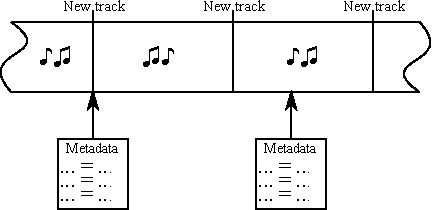
\includegraphics{stream}
\end{center}
 \caption{A \liquidsoap{} stream}
 % Stream.png: 500x132 pixel, 91dpi, 14.03x3.70 cm, bb=0 0 398 105
\end{figure}

One may also want to change the metadata of the stream,
to display informations about the radio, or execute a script on each metadata 
in order, for instance, to keep track of the songs that are being played and 
display this information on a website. This can be done using the following code:
\begin{verbatim}
 def f(m) = 
    title  = m["title"]
    system("/path/to/script #{quote(title)}")
 end
 s = on_metadata(f, s)
 def new_metadata(m) = 
    title  = m["title"]
    [("title","#{title} -- My Radio !")]
 end
 s = map_metadata(new_metadata, s)
\end{verbatim}
The above code is an example of the need for a functional language to build multimedia 
streams. Indeed, streams are infinite objects, hence, it is not possible to specify in advance
the full data stream. For this reason, the \liquidsoap{} languages uses operators that take 
a function as parameter and apply this function when the relevant data is available, here 
a metadata.

Passing functions as arguments is not the only functional aspect of \liquidsoap{}. The language is 
also \textit{statically typed} and the types are \textit{inferred}. Static types are important to 
assure a consistency of the stream while the inferrence hides most of these aspects to 
the final user which, as said before, is usually not a programming expert.

We conclude this presentation with another example. When building a source composed
of a lives shows and local files, one may want, for instance, to play a jingle when starting
or stopping the live shows. Additionally, one may also want to fade the 
end of the live and the beginning of the playlist. This can be done using \texttt{transitions}:
\begin{verbatim}
 def transition(old,new) = 
    jingle = single("/path/to/jingle.mp3")])
    sequence([fade.out(old), 
              jingle, 
              fade.in(new)])
 end
 s = fallback(transitions=[transition,transition], 
                          [live,files])
\end{verbatim}
In this example, the user defines a function that takes the old and new sources and combine them
to create the required transition. In our case, the transition consists of fade out the old 
source, then play a jingle and finally fade in the new source. As for the metadata operators,
the transition function is passed as an argument for the fallback operator and applied 
each time the operator needs to switch from one source to another.

With this brief presentation of the \liquidsoap{} language, we have seen in very simple and 
concise examples how to build a custom multimedia stream using operators of the language. 
The possibilities offered by the use of a programming 
language are vast. These features make \liquidsoap{} a language very attractive for users
interested in building their custom stream where the usual tools do not provide 
enough flexibility to fit their need.
\bibliographystyle{abbrv}
\bibliography{biblio}
\end{document}
